\documentclass[convert={density=150x150},border={10pt 10pt 10pt 10pt}]{standalone}
\usepackage{amsmath, amssymb, amsthm}
\usepackage{tikz}
\usetikzlibrary{arrows,shapes,snakes,automata,backgrounds,petri}
\tikzset{n/.style={inner sep=0, minimum size=6pt, fill=black, circle}}
\begin{document}
\pagecolor{white}
  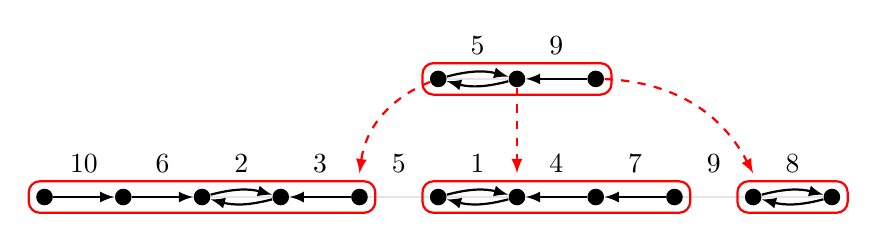
\begin{tikzpicture}
    \foreach \x in {0,1,...,10}
    {
      \node[n](A\x) at (\x, 0) {};
    }
    \def\testarray{{10,6,2,3,5,1,4,7,9,8}}
    \foreach \x in {0,1,...,9}
    {
      \pgfmathparse{int(\x+1)}
      \edef\y{\pgfmathresult}%
      \pgfmathparse{\testarray[\x]}
      \edef\v{\pgfmathresult}
      \draw[black!10,thick] (A\x) -- (A\y) node [black, midway, above, yshift=5pt] {$\v$};
    }
    \foreach \x in {0,1} {
      \pgfmathparse{int(\x+1)}
      \edef\y{\pgfmathresult}%
      \draw[-latex,thick] (A\x) edge (A\y);
    }
    \foreach \x in {2,5,9} {
      \pgfmathparse{int(\x+1)}
      \edef\y{\pgfmathresult}%
      \draw[-latex,thick] (A\x) edge [bend left=15] (A\y);
      \draw[-latex,thick] (A\y) edge [bend left=15] (A\x);
    }
    \foreach \x in {3,6,7} {
      \pgfmathparse{int(\x+1)}
      \edef\y{\pgfmathresult}%
      \draw[-latex,thick] (A\y) edge (A\x);
    }
    \draw[rounded corners,draw=red,thick] (-0.2, -0.2) rectangle (4.2, 0.2);
    \draw[rounded corners,draw=red,thick] (4.8, -0.2) rectangle (8.2, 0.2);
    \draw[rounded corners,draw=red,thick] (8.8, -0.2) rectangle (10.2, 0.2);


    \node[n](B1) at (5, 1.5) {};
    \node[n](B2) at (6, 1.5) {};
    \node[n](B3) at (7, 1.5) {};
    \draw[thick, dashed, draw=red, -latex](B1) edge [red, bend right] (4, 0.3);
    \draw[thick, dashed, draw=red, -latex](B2)-- (6, 0.3);
    \draw[thick, dashed, draw=red, -latex](B3) edge [red, bend left] (9, 0.3);
    \draw[black!10,thick] (B1)--(B2) node[black, midway, above, yshift=5pt] {$5$};
    \draw[thick] (B1) edge[bend left=15, -latex] (B2);
    \draw[thick] (B2) edge[bend left=15, -latex] (B1);
    \draw[thick, -latex] (B3) -- (B2) node[midway, above, yshift=5pt] {$9$};
    \draw[rounded corners,draw=red,thick] (4.8, 1.3) rectangle (7.2, 1.7);
  \end{tikzpicture}
\end{document}